\documentclass[10pt,twocolumn]{article}

\usepackage[margin=0.72in,columnsep=0.24in]{geometry}
\usepackage[T1]{fontenc}
\usepackage{lmodern}
\usepackage{microtype}
\usepackage{amsmath,amssymb,amsthm}
\usepackage{booktabs,multirow}
\usepackage{enumitem}
\usepackage{graphicx}
\usepackage{tikz}
\usetikzlibrary{arrows.meta,positioning,fit}
\usepackage{xcolor}
\definecolor{accent}{HTML}{274C77}
\definecolor{softgray}{HTML}{F2F3F5}
\usepackage[colorlinks=true,allcolors=accent]{hyperref}
\usepackage[nameinlink,capitalise]{cleveref}
\usepackage{natbib}
\usepackage{url}

\newtheorem{proposition}{Proposition}
\newtheorem{definition}{Definition}
\newcommand{\ind}{\mathbb{I}}
\newcommand{\botans}{\bot}
\newcommand{\method}{\textsc{CEA}}
\newcommand{\dataset}{\textsc{CEval-32}}

\title{Beyond Citation Entailment: Causal Evidence Audits for Retrieval-Augmented Language Models}
\author{Sergio Luiz Wermuth Figueras}
\date{}

\begin{document}
\maketitle

\begin{abstract}
Retrieval-augmented language models and deep-research agents are commonly evaluated by answer correctness and by whether cited passages support generated claims. These observations establish compatibility between an answer and its citations, but they do not establish that the cited evidence determined the answer. A system can answer from parametric memory, a positional shortcut, or a prior draft and attach an entailing citation afterward. We introduce the \emph{Causal Evidence Audit} (\method), a black-box evaluation protocol that complements citation entailment with three controlled tests: paired-world responsiveness when one decisive fact changes, abstention when indispensable evidence is removed, and proof-chain citation coverage. We show constructively that causal grounding is not identifiable from any single-world observational citation score. We then instantiate the protocol in \dataset, a transparent pilot of 32 fictional-entity items spanning direct lookup, two-hop composition, numerical comparison, and conditional reasoning. Two locally executed open-weight models, each tested with ordinary and evidence-contract prompts, produced 384 greedy-decoded generations. Single-world observational pass rates ranged from 59.4\% to 78.1\%, whereas the coverage-based joint causal score ranged from 0\% to 31.3\%; the strict score, which also rejects extraneous citations, ranged from 0\% to 31.3\%. Stronger grounding instructions sometimes increased the observational score while decreasing the strict causal score. We additionally specify \emph{CEA-Extended} (dataset schema v2): multiple decisive edits, answer-preserving perturbations, alternative proof sets, sufficient-evidence ablations, and policy-governed conflicts, with a separate retrieval-stage audit. These extensions are proposed and have no new model results here. A finite black-box audit cannot certify universal reliance. The pilot demonstrates that commonly reported citation success can conceal unsupported guessing and post-hoc attribution, and motivates paired evidence interventions as an evaluation layer for high-stakes RAG and research agents.
\end{abstract}

\section{Introduction}

Retrieval-augmented generation (RAG) was introduced to combine parametric language modeling with external, updateable knowledge \citep{lewis2020rag}. The basic promise is operationally important: retrieve relevant evidence, generate an answer conditioned on it, and expose sources that a reader can inspect. Browser-assisted systems such as WebGPT \citep{nakano2021webgpt} and evidence-producing models such as GopherCite \citep{menick2022verified} made citations a central interface for trustworthy language generation. The same pattern now underlies long-form research agents, which browse, synthesize, and produce citation-rich reports.

Evaluation has largely followed the visible artifact. Attributable to Identified Sources (AIS) asks whether generated statements are supported by identified sources \citep{rashkin2021ais}. Audits of generative search measure citation completeness and citation correctness \citep{liu2023verifiability}; ALCE evaluates fluency, answer correctness, and citation quality \citep{gao2023alce}. RAGAS, ARES, and RAGCHECKER decompose retrieval relevance, faithfulness, and answer quality in increasingly fine-grained ways \citep{es2023ragas,saadfalcon2023ares,ru2024ragchecker}. These are necessary measurements. They answer whether the output is consistent with the presented evidence and whether a reader can verify it.

They do not, by themselves, answer a different question: \emph{did the system's answer depend on the evidence it cites?} An entailing citation can be attached after an answer has already been produced. A model may ignore a decisive passage, follow a familiar prior, select the first document, or guess under missing evidence while still producing a citation that looks appropriate. Recent work makes the distinction increasingly consequential. ContextCite and RAGONITE use context removal to estimate which evidence contributed to a generation \citep{cohenwang2024contextcite,saharoy2024ragonite}. Counterfactual prompting and set-level verification have been used for RAG risk control and selective abstention \citep{chen2024risk,qiu2026surerag}, while leave-one-out changes can reveal poisoned documents \citep{kumar2026raguard}. Deceptive Grounding shows that real citations and high measured faithfulness can coexist with entity-attribution failure \citep{caruzzo2026deceptive}. Work on knowledge conflicts further shows that models may integrate evidence unevenly or positionally \citep{xu2024knowledge,yang2026contextconflict}. Meanwhile, evaluations of deep-research agents identify evidence integration and dependency-consistent reasoning as persistent bottlenecks \citep{zhang2025finder,guo2026mrlhdr}.

This paper argues that grounding evaluation needs both \emph{observational support} and \emph{interventional reliance}. We propose \method, a model-agnostic protocol built around matched evidence worlds. In a paired item, exactly one answer-determining proposition is changed; nuisance content is either held fixed or modified by a predeclared, answer-invariant balancing edit. A grounded system must change its answer accordingly. In a matched ablation, indispensable evidence is removed; a grounded system must abstain rather than complete the missing link from a shortcut. Citations are then checked against the oracle proof set in each world.

The contributions are:
\begin{enumerate}[leftmargin=*,itemsep=2pt,topsep=3pt]
    \item a formal separation between semantic citation support and causal evidence reliance, including a constructive non-identifiability result for single-world observational metrics;
    \item a black-box audit protocol and joint metrics that combine paired-world responsiveness, necessity-aware abstention, and proof-chain citation alignment;
    \item \dataset, a reproducible 32-item pilot with fictional entities and four reasoning families, together with 384 raw generations from two quantized open-weight models under two prompting regimes; and
    \item a versioned extension with multiple interventions, admissible alternative proofs, conflict policies, separate retrieval checks, and an explicit limit on finite black-box certification; and
    \item an intervention-based training objective and reporting checklist for real retrieval corpora and long-horizon research agents.
\end{enumerate}

The empirical study is intentionally labeled a pilot. Its purpose is to test whether the proposed measurements reveal behavior hidden by a single-world score, not to rank model families or establish population-level performance.

\section{Related Work}

\subsection{Attribution and RAG evaluation}

AIS formalized whether a statement is attributable to identified sources and validated a human annotation procedure across generation tasks \citep{rashkin2021ais}. Generative-search audits subsequently operationalized citation recall and precision, finding substantial gaps despite fluent answers \citep{liu2023verifiability}. ALCE provided reproducible citation evaluation over several long-form question-answering settings \citep{gao2023alce}. RAGAS evaluates RAG pipelines without reference answers \citep{es2023ragas}; ARES trains lightweight judges with synthetic data and uses prediction-powered inference \citep{saadfalcon2023ares}; RAGCHECKER diagnoses retriever and generator failure modes at claim level \citep{ru2024ragchecker}. These methods estimate support, relevance, utilization, or human preference from observed inputs and outputs.

Citation generation can occur with the answer or after it. A recent comparison reports a coverage--correctness trade-off between generation-time and post-hoc citation paradigms \citep{saxena2025citation}. That result makes reliance especially important: if a citation is selected after drafting, semantic support does not imply that the source influenced the draft. \method{} is agnostic to when citations are produced and tests the completed system under controlled evidence changes.

\subsection{Context attribution and interventions}

ContextCite attributes a generated statement to parts of the context using a sparse surrogate trained on context ablations \citep{cohenwang2024contextcite}. RAGONITE similarly computes counterfactual attribution by comparing a response with the response obtained after removing evidence \citep{saharoy2024ragonite}. Their central intuition---removing a causally relevant source should affect the response---is aligned with this work. Our focus is complementary: rather than estimate a contribution for an already generated statement, \method{} defines an end-to-end evaluation contract across two coherent answer-changing worlds, a necessary-evidence ablation, oracle answers and proof sets, and the citations emitted in each world.

Counterfactual methods have also been used to estimate RAG risk and encourage abstention \citep{chen2024risk}. SURE-RAG treats evidence sufficiency as a set-level property and evaluates a selective verifier with counterfactual swaps and no-oracle controls \citep{qiu2026surerag}. RAGuard uses leave-one-out decoding as one layer of a poisoning defense \citep{kumar2026raguard}. Attribution-bias studies intervene on source authorship metadata and show that attribution changes under nominally irrelevant cues \citep{abolghasemi2024bias}. Deceptive Grounding isolates entity-attribution failures that remain invisible to conventional faithfulness and citation checks \citep{caruzzo2026deceptive}. These works establish that counterfactual removal, sufficiency verification, abstention, and attribution failure are not individually new. To our knowledge, prior protocols do not make correct behavior in both minimally different answer worlds, abstention after removing an indispensable proof element, and oracle proof-chain citations a single per-item pass condition. \method{} targets that joint behavioral contract.

Counterfactual evaluation has a longer history in knowledge updating. MQuAKE asks whether edited facts propagate to multi-hop consequences \citep{zhong2023mquake}; ReCoE broadens counterfactual editing to multiple reasoning schemes \citep{hua2024recoe}. Those benchmarks evaluate changes to model knowledge. \method{} instead intervenes on inference-time evidence and does not modify model weights.

\subsection{Research agents and evidence integration}

DeepResearch Bench assesses expert-level report tasks, effective citations, and citation accuracy \citep{du2025deepresearch}. ReportBench checks cited-statement consistency and non-cited factuality in generated surveys \citep{li2025reportbench}. FINDER and its failure taxonomy identify evidence integration, verification, and resilient planning as core weaknesses \citep{zhang2025finder}. Mr.LHDR extends evaluation to long, multimodal dependency graphs and reports a large gap between final-answer accuracy and strict dependency-consistent success \citep{guo2026mrlhdr}. These findings motivate an audit that can localize whether a research conclusion follows its decisive evidence. \method{} is designed as an additional layer for such benchmarks, not as a replacement for coverage, writing quality, source authority, or factuality evaluation.

\section{Why Citation Support Is Not Enough}

\subsection{Problem setting}

Let $q$ be a query and $E=(e_1,\ldots,e_m)$ an ordered evidence bundle. A system $A$ returns an answer and a citation set,
\begin{equation}
    A(q,E)=(\hat y, C), \qquad C\subseteq\{1,\ldots,m\}.
\end{equation}
Let $y^*(q,E)$ be the oracle answer, and let $G(q,E)$ be a minimal oracle proof set: the document indices required to derive $y^*$ under the benchmark semantics. The abstention symbol $\botans$ denotes that $E$ does not determine a unique answer.

An observational support evaluator sees one realized tuple $(q,E,\hat y,C)$. It may assess correctness, whether $E_C$ entails $\hat y$, whether all answer claims are cited, and whether citations are relevant. These properties are functions of the realized artifact. Evidence reliance is a property of the mapping $E\mapsto A(q,E)$ across possible evidence worlds.

\begin{definition}[Observational citation support]
For a support predicate $S$, an output is observationally supported when $S(q,E,\hat y,C)=1$. The predicate may be implemented by humans, natural-language inference, an LLM judge, or a controlled proof oracle.
\end{definition}

\begin{definition}[Interventional evidence responsiveness]
For a valid intervention $T$ that changes answer-determining evidence, a system is responsive on $(q,E,T)$ when its output changes to the oracle answer for $T(E)$ while remaining correct on $E$.
\end{definition}

\subsection{A non-identifiability result}

\begin{proposition}[Single-world non-identifiability]
No evaluator that observes only $(q,E_0,\hat y,C)$ in one evidence world can, without additional assumptions, identify whether $\hat y$ causally depends on $E_0$.
\end{proposition}

\begin{proof}
Fix an observed world $E_0$ with oracle answer $y_0$ and an entailing citation set $C_0$. Construct a responsive system $A_R$ that computes $y^*(q,E)$ and cites its proof set. Construct a post-hoc system $A_P$ that returns the memorized answer $y_0$ and attaches $C_0$ whenever evaluated at $E_0$. The two systems induce the same observed tuple at $E_0$, so every evaluator restricted to that tuple assigns the same score. Now choose a valid intervention $T$ with $y^*(q,T(E_0))=y_1\neq y_0$. By construction, $A_R$ returns $y_1$, while $A_P$ can continue returning $y_0$. Their evidence reliance differs although their single-world observation is identical. Therefore reliance is not identifiable from that observation alone.
\end{proof}

The proposition does not say observational metrics are unhelpful. It says they identify a different property. Entailment protects the reader against unsupported claims in the displayed artifact; intervention tests whether the system behavior is governed by the evidence. A trustworthy evidence-using system needs both.

\begin{proposition}[Finite black-box audits do not certify universal reliance]
\label{prop:finite}
Let $\mathcal{X}$ be an evidence-world domain containing a valid world outside a finite set $Q$ queried by an audit. Without restrictions on the audited system's function class, passing every query in $Q$ does not imply correct evidence reliance on every world in $\mathcal{X}$. This also holds when the finite queries are chosen adaptively.
\end{proposition}

\begin{proof}
Let $A_R$ return the oracle answer and an admissible proof in every answerable world, and abstain in every insufficient world. Run the finite audit against $A_R$ and call its queried set $Q$. Choose $x^*\in\mathcal{X}\setminus Q$. Define $A_B(x)=A_R(x)$ for all $x\neq x^*$, but at $x^*$ let $A_B$ output an incorrect answer, an unsupported citation, or a non-abstaining guess. Because the audit observes the same answer and citations at every query in $Q$, it follows the same adaptive path and gives $A_B$ the same score as $A_R$. Yet $A_B$ fails at $x^*$. Randomization changes the probability of encountering $x^*$, not the logical implication from a finite realized transcript to universal correctness.
\end{proof}

The result concerns unrestricted black-box systems over non-exhaustively tested domains. It does not rule out population estimates with a declared sampling design, guarantees under explicit structural assumptions, or exhaustive testing of a genuinely finite domain. It also does not identify internal neural mechanisms: the audit establishes behavior on sampled interventions.

\section{The Causal Evidence Audit}

\subsection{Matched evidence worlds}

For each base item, an audit author specifies a query $q$, two evidence worlds $E^{(0)}$ and $E^{(1)}$, distinct oracle answers $y^{(0)}$ and $y^{(1)}$, and oracle proof sets $G^{(0)}$ and $G^{(1)}$. The worlds differ by a minimal, answer-determining edit $T$ such that
\begin{equation}
 E^{(1)}=T(E^{(0)}), \qquad y^{(1)}\neq y^{(0)}.
\end{equation}
All non-causal features that can feasibly be controlled---document count, style, entity frequency, answer mention frequency, and ordering---should remain fixed or be explicitly balanced by an answer-invariant edit whose role is documented.

The audit also constructs an ablated world $E^{(-)}$ by removing an indispensable proof element from $E^{(0)}$. The oracle answer is then $\botans$. An optional nuisance intervention $P$ permutes irrelevant documents or changes non-semantic metadata while preserving the oracle answer. This fourth condition tests selective invariance, but it was not included in the pilot.

\begin{figure}[t]
\centering
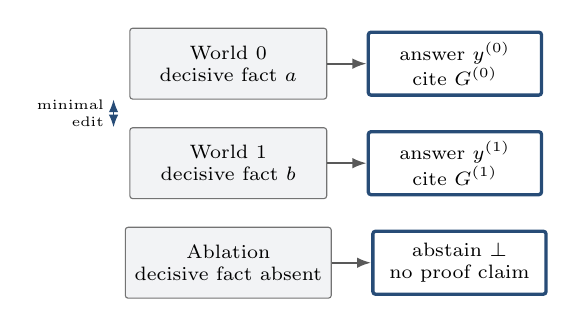
\begin{tikzpicture}[
    node distance=3.5mm and 5mm,
    box/.style={draw=black!55,rounded corners=1pt,fill=softgray,align=center,font=\scriptsize,minimum width=25mm,minimum height=9mm},
    resultbox/.style={draw=accent,very thick,rounded corners=1pt,align=center,font=\scriptsize,minimum width=22mm,minimum height=8mm},
    arr/.style={-{Latex[length=1.8mm]},thick,draw=black!65}
]
\node[box] (w0) {World 0\\decisive fact $a$};
\node[resultbox,right=of w0] (a0) {answer $y^{(0)}$\\cite $G^{(0)}$};
\node[box,below=of w0] (w1) {World 1\\decisive fact $b$};
\node[resultbox,right=of w1] (a1) {answer $y^{(1)}$\\cite $G^{(1)}$};
\node[box,below=of w1] (wm) {Ablation\\decisive fact absent};
\node[resultbox,right=of wm] (am) {abstain $\botans$\\no proof claim};
\draw[arr] (w0)--(a0);
\draw[arr] (w1)--(a1);
\draw[arr] (wm)--(am);
\draw[{Latex[length=1.6mm]}-{Latex[length=1.6mm]},dashed,draw=accent] ([xshift=-2mm]w0.south west)--node[left,font=\tiny,align=right]{minimal\\edit} ([xshift=-2mm]w1.north west);
\end{tikzpicture}
\caption{A three-condition Causal Evidence Audit. Passing requires correct behavior in all matched worlds, not merely an entailing citation in one world.}
\label{fig:audit}
\end{figure}

\subsection{Metrics}

Let $(\hat y^{(w)},C^{(w)})=A(q,E^{(w)})$. Exact answer matching can be replaced by a task-appropriate semantic judge, provided the judge is fixed before evaluation.

\paragraph{Counterfactual response consistency.}
\begin{equation}
\mathrm{CRC}_i=\ind[\hat y_i^{(0)}=y_i^{(0)}\;\wedge\;\hat y_i^{(1)}=y_i^{(1)}].
\end{equation}
Because the two oracle answers differ, this tests a correct answer switch rather than mere output instability.

\paragraph{Evidence-necessity abstention.}
\begin{equation}
\mathrm{ENA}_i=\ind[\hat y_i^{(-)}=\botans].
\end{equation}
ENA penalizes filling an evidence gap with an unsupported answer. It is not a generic refusal metric: abstention is correct only in the matched ablation world.

\paragraph{Proof citation precision and recall.}
For $w\in\{0,1\}$,
\begin{align}
 \mathrm{PCR}_i^{(w)} &= \frac{|C_i^{(w)}\cap G_i^{(w)}|}{|G_i^{(w)}|},\\
 \mathrm{PCP}_i^{(w)} &= \frac{|C_i^{(w)}\cap G_i^{(w)}|}{|C_i^{(w)}|},
\end{align}
with PCP defined as zero for an empty citation set when $G$ is nonempty. PCR asks whether every necessary proof document is cited; PCP penalizes extraneous citations. Let $V_i^{(-)}$ indicate that every citation emitted in the ablated world names a document actually present in that world. Span-level proof sets should be preferred when reliable annotations are available.

\paragraph{Joint scores.}
The coverage-based score is a hard per-item pass:
\begin{equation}
\mathrm{CES}^{\mathrm{cov}}_i=\mathrm{CRC}_i\,\mathrm{ENA}_i\,V_i^{(-)}
\prod_{w\in\{0,1\}}\ind[\mathrm{PCR}_i^{(w)}=1].
\end{equation}
The strict score additionally requires exact proof citations in both full worlds and no proof citation after abstention:
\begin{equation}
\begin{aligned}
\mathrm{CES}^{\mathrm{strict}}_i={}&\mathrm{CRC}_i\,\mathrm{ENA}_i\,V_i^{(-)}
\ind[C_i^{(-)}=\varnothing]\\
&\times\prod_{w\in\{0,1\}}\ind[C_i^{(w)}=G_i^{(w)}].
\end{aligned}
\end{equation}
Dataset scores are macro-averages over items. The multiplicative construction is intentional: high answer accuracy cannot compensate for guessing when evidence is absent, and citation verbosity cannot compensate for omitting a necessary proof link.

\paragraph{Single-world observational pass.}
For comparison, the pilot reports
\begin{equation}
\mathrm{OBS}_i=\ind[\hat y_i^{(0)}=y_i^{(0)}]\ind[\mathrm{PCR}_i^{(0)}=1].
\end{equation}
OBS is a controlled proxy for the common pattern ``correct answer plus complete supporting citations.'' It is not claimed to reproduce every existing attribution metric.

\subsection{Audit validity requirements}

An intervention is only informative if the counterfactual world is coherent and the edit is truly answer-determining. We recommend five construction gates:
\begin{enumerate}[leftmargin=*,itemsep=1pt,topsep=3pt]
    \item \textbf{Minimality:} change the fewest atomic propositions consistent with a coherent alternative world.
    \item \textbf{Answer separation:} independently verify that the oracle answers differ.
    \item \textbf{Proof completeness:} annotate all necessary sources, including multi-hop links.
    \item \textbf{Nuisance balance:} control position, length, lexical overlap, source style, and answer-mention frequency.
    \item \textbf{Ablation validity:} confirm that removal makes the answer underdetermined rather than merely harder.
\end{enumerate}
For open-web agents, exact control is difficult. A practical alternative is to freeze a retrieved snapshot, perform document-level or claim-level interventions inside the snapshot, and evaluate the synthesis stage separately from retrieval. End-to-end retrieval interventions can then be added as a second layer.

\section{CEA-Extended (schema v2)}
\label{sec:extended}

The preceding definitions and all pilot numbers belong to the original three-condition CEA protocol, preserved as \emph{paper-v0.1}. This section specifies \emph{CEA-Extended} (dataset schema v2) as a prospective protocol. Its deterministic construction fixtures test the specification, not any language model. No CEval-32 item, archived generation, or published pilot aggregate is rescored here.

\subsection{Evidence sufficiency and alternative proofs}

Under a preregistered domain semantics and conflict policy $\pi$, let
$\mathcal{G}_{\pi}(q,E,a)$ be the family of all annotated, inclusion-minimal,
admissible document sets sufficient to establish answer $a$ in world $E$.
Documents have stable identifiers across edits and reorderings; for
contradictory claims, $\pi$ determines which sources are admissible. Define
$y^*_{\pi}(q,E)=a$ only if exactly one answer is established after applying
$\pi$; otherwise $y^*_{\pi}(q,E)=\botans$. A family with two independent
proofs, such as $\{\{D1,D2\},\{D3,D4\}\}$, represents genuine redundancy,
not a four-document conjunctive proof. Write $\mathcal{G}_w(a)$ for
$\mathcal{G}_{\pi}(q,E^{(w)},a)$. For an answerable world, the two
citation contracts are
\begin{align}
\mathrm{Cov}_{w}(C,a)
 &= \ind[C\subseteq\mathrm{IDs}(E^{(w)})]\,
    \ind[\exists G\in\mathcal{G}_w(a):G\subseteq C],\\
\mathrm{Exact}_{w}(C,a)
 &= \ind[C\in\mathcal{G}_w(a)].
\end{align}
The coverage contract permits extra present citations, whereas the exact
contract accepts \emph{one} complete minimal proof and rejects both missing
links and citation padding. Neither requires citing the union of alternative
proofs. An abstention has an empty citation set in the exact contract.
These definitions replace the single-gold-set citation rule only in
CEA-Extended; they do not retroactively change pilot PCR, PCP, or CES.

\subsection{Predeclared intervention families}

For each base item, construct a finite, versioned family of worlds and
record the expected answer and all admissible minimal proofs for each:
\begin{enumerate}[leftmargin=*,itemsep=1pt,topsep=3pt]
    \item \textbf{Multiple decisive edits:} create at least two independently designed coherent edits $T_1,\ldots,T_K$ ($K\geq2$), each with $y^*_{\pi}(q,T_k(E^{(0)}))\neq y^*_{\pi}(q,E^{(0)})$. Record changed propositions and control answer-token and position cues. The edits need not have mutually distinct alternative answers.
    \item \textbf{Answer-preserving perturbations:} vary document order, irrelevant metadata, distractor wording, or non-decisive facts through $P_j$ while checking $y^*_{\pi}(q,P_j(E^{(0)}))=y^*_{\pi}(q,E^{(0)})$. Correctness and an admissible proof are required; identical citation IDs are not required if more than one proof remains valid.
    \item \textbf{Two ablation classes:} a \emph{necessity} removal $R_\bot$ must eliminate every admissible proof and make the answer underdetermined; the correct output is $\botans$. A \emph{redundancy} removal $R_+$ deletes one proof path while leaving another complete path; the correct output remains the answer with a surviving proof. The oracle, not the mere act of removal, assigns the expected behavior.
    \item \textbf{Policy-governed conflicts:} insert incompatible claims in a coherent snapshot and apply a fixed policy $\pi$ for source authority, version, or time. A uniquely preferred admissible proof gives its answer; an unresolved tie yields $\botans$. The policy and provenance must be fixed before outputs are observed.
\end{enumerate}
The schema-v2 validator requires one baseline, at least two decisive
counterfactuals, and at least one nuisance, necessity ablation, redundancy
ablation, and conflict condition per case. This checks role completeness and
stable IDs; it cannot replace expert semantic review of the documents.
Let $\mathcal{W}^{+}_i$ contain the answerable base, decisive,
perturbation, redundancy, and resolved-conflict worlds, and let
$\mathcal{W}^{\bot}_i$ contain only independently verified insufficient
necessity and unresolved-conflict worlds. Let $a_w=\ind[\hat y^{(w)}
=y^*_{\pi}(q,E^{(w)})]$ and let $f_w$ indicate that the response
obeys the declared answer-and-citation output schema. For an answerable
world, $c_{\mathrm{cov}}(w)$
and $c_{\mathrm{exact}}(w)$ are the citation contracts above. For an
insufficient world, let $c_{\mathrm{cov}}(w)=\ind[C^{(w)}
\subseteq\mathrm{IDs}(E^{(w)})]$ and
$c_{\mathrm{exact}}(w)=\ind[C^{(w)}=\varnothing]$. The prospective joint
criterion for $s\in\{\mathrm{cov},\mathrm{exact}\}$ is
\begin{equation}
\mathrm{CES}^{(2,s)}_i=
\prod_{w\in\mathcal{W}^{+}_i\cup\mathcal{W}^{\bot}_i}
a_w\,f_w\,c_s(w).
\end{equation}
Report component rates by intervention class and the joint pass rate; a hard
product alone does not reveal which failure occurred. Evaluate stochastic
systems with a declared number of repeated runs and aggregate at the item
level, retaining the observed run-to-run spread.

\subsection{Oracle and ablation validity gates}

A case enters the score only after independent annotators or a trusted
domain oracle establish: (i) that each edited world is internally coherent
and differs only in predeclared propositions; (ii) that the query has the
annotated answer under $\pi$; (iii) that every annotated proof is sufficient
and inclusion-minimal; and (iv) that no unannotated alternate proof remains
after a necessity ablation. For complex corpora, dual annotation,
disagreement adjudication, and targeted search for surviving proofs reduce
oracle error. If a removal leaves another complete derivation, classify it
as a redundancy world rather than scoring abstention. If source authority
cannot be resolved under $\pi$, annotate insufficiency explicitly rather
than silently choosing one claim. Invalid worlds are excluded with reasons,
not converted to model failures.

\subsection{A separate retrieval-stage audit}

The fixed-bundle experiment tests generation conditioned on supplied
evidence. To test retrieval, make coherent edits to a frozen corpus
snapshot, rerun indexing and retrieval with the same query and declared
configuration, and inspect the returned evidence before generation. Record
whether an admissible proof is available in the corpus, whether the
retriever returns a complete admissible proof within the fixed budget, and
whether the final answer satisfies the conditional synthesis contract.
An end-to-end failure can then be attributed to missing corpus evidence,
retrieval miss, or generation/citation error. Equivalent documents that
survive an edit must count as legitimate recovery. Report the fixed-bundle,
retrieval, and end-to-end results separately; a synthesis-only result is
never labeled an end-to-end RAG result.

\subsection{Generalization and interpretation}

Pre-register the intervention generator and scoring code, then evaluate on
held-out templates, entities, answer values, proof-graph shapes, domains,
and source styles. Keep systems being tuned away from the private final
items, and publish failure modes plus confidence intervals using the
actual sampling unit. A per-case Wilson interval, as in the current
runner, describes item-level variation only; correlated templates or
domains require a grouped bootstrap or hierarchical analysis beyond
this fixture. Perturbations should include unseen combinations,
not just paraphrases of training templates. A high score is evidence of
reliance \emph{under the tested distribution and policy}; it cannot prove
universal reliance or reveal internal mechanisms
(\cref{prop:finite}). Source truth and policy legitimacy remain separate
questions.

\section{Pilot Study}

\subsection{Research questions}

The pilot addresses three narrow questions:
\begin{enumerate}[label=\textbf{RQ\arabic*.},leftmargin=*,itemsep=2pt,topsep=3pt]
    \item Does paired intervention expose a gap hidden by a single-world observational pass?
    \item Is missing-evidence abstention a distinct bottleneck from following a changed fact?
    \item Does a stronger evidence-contract prompt reliably improve the joint score?
\end{enumerate}

\subsection{Dataset}

\dataset{} contains 32 items, eight in each of four reasoning families:
\begin{itemize}[leftmargin=*,itemsep=1pt,topsep=3pt]
    \item \textbf{Direct lookup:} one registry sentence determines a fictional reactor's authorized coolant.
    \item \textbf{Two-hop composition:} a dispatch ledger selects a depot, and a second source maps the depot to a cipher.
    \item \textbf{Numerical comparison:} two verified values and a ranking rule determine the higher-ranked fictional station.
    \item \textbf{Conditional reasoning:} a threshold policy and a site measurement determine a required protocol.
\end{itemize}
All entity and value names were constructed for the benchmark. This reduces the opportunity to answer from memorized world knowledge. For each item, world 1 changes one decisive sentence or number from world 0. In the direct, two-hop, and conditional families, all other documents are unchanged. In the comparison family, the explicitly obsolete value in D4 also swaps high and low tokens to preserve the numerical multiset across worlds; D4 is excluded from the oracle proof and does not affect the answer under the benchmark semantics. The ablation removes the decisive document from world 0. Distractors include obsolete estimates, preliminary trials, availability statements, and non-diagnostic descriptions. The benchmark file records both worlds, expected answers, gold citation sets, and the ablation target.

\subsection{Models and prompting regimes}

We evaluated the 4-bit MLX conversions \texttt{mlx-community/Qwen3-4B-4bit} and \texttt{mlx-community/Llama-3.2-3B-Instruct-4bit}. Qwen3 is documented in \citet{yang2025qwen3}, while the exact Llama-3.2-3B-Instruct release is documented by its model card \citep{meta2024llama32}. The two evaluated MLX conversion artifacts are identified separately \citep{mlxcommunity2025qwen3,mlxcommunity2024llama32}, and their immutable revisions are recorded in the public repository. Quantized conversions may not reproduce full-precision behavior, so these identifiers are part of the experimental specification rather than incidental details.

Each model was tested under two system prompts. The \emph{baseline} required use of numbered sources, abstention when sources were insufficient, and a JSON answer with citation IDs. The \emph{evidence contract} additionally required the model to identify internally the smallest complete proof chain, answer only when every necessary link was explicit, and cite every proof source without irrelevant citations. Full prompts appear in \cref{app:prompts}.

The design comprises $32\times 3\times 2\times 2=384$ generations: 32 items, three evidence conditions, two models, and two regimes. Decoding was greedy (temperature zero) with a 96-token maximum. All inference was local through MLX; no external API was used. The release run used Python 3.14.6 on a 14-core Apple M4 Pro with 48~GB memory, running macOS 26.5.2, MLX 0.32.2, MLX-LM 0.31.3, and Transformers 5.17.0. The experiment script writes the generated benchmark, per-model raw responses, summary metrics, and a machine-readable provenance manifest with source and artifact hashes.

\paragraph{Code and artifacts.}
The complete source code for the tests is available at \url{https://github.com/sergiofigueras/causal-evidence-audit}; the immutable artifact release is \url{https://github.com/sergiofigueras/causal-evidence-audit/releases/tag/v0.1.0}. The repository contains the benchmark generator, the realized 32-item benchmark, both system prompts, all 384 raw generations, machine-readable summaries, model identifiers and revisions, a hash-locked environment, validation code, and execution instructions.

\subsection{Scoring and uncertainty}

Answers were normalized for case and punctuation. A response counted as correct if it contained exactly the expected fictional candidate and not the alternative; wrapper phrases such as ``Protocol X'' were allowed. Abstentions were recognized from a fixed list including \texttt{INSUFFICIENT}, ``not specified,'' and ``cannot determine.'' Citation IDs were validated against the JSON schema. Gold proof coverage required every annotated proof source; strict matching rejected both missing and extraneous sources.

We report Wilson 95\% confidence intervals for binary proportions. These intervals quantify sampling uncertainty over the 32 templated items, not uncertainty over prompts, decoders, model versions, domains, or natural document distributions. No null-hypothesis significance tests are reported because the pilot was designed for diagnostic demonstration, not comparative model inference.

\section{Results}

\begin{table*}[t]
\centering
\small
\setlength{\tabcolsep}{5.2pt}
\caption{Pilot results on 32 items per model and prompt regime. W0/W1 are answer accuracy in the paired worlds; CRC is paired response consistency; ENA is evidence-necessity abstention; OBS is the single-world observational pass; CES$^{\mathrm{cov}}$ requires correct switching, valid ablation citations, ablation abstention, and complete proof citations in both worlds; CES$^{\mathrm{strict}}$ also rejects extraneous full-world citations and any ablation citation. Values are percentages.}
\label{tab:main}
\begin{tabular}{llrrrrrrr}
\toprule
Model & Prompt & W0 & W1 & CRC & ENA & OBS & CES$^{\mathrm{cov}}$ & CES$^{\mathrm{strict}}$\\
\midrule
Qwen3-4B & Baseline & 87.5 & 100.0 & 87.5 & 31.3 & 75.0 & 31.3 & 31.3\\
Qwen3-4B & Evidence contract & 87.5 & 100.0 & 87.5 & 6.3 & \textbf{78.1} & 6.3 & 0.0\\
Llama-3.2-3B & Baseline & 93.8 & 93.8 & \textbf{87.5} & 0.0 & 59.4 & 0.0 & 0.0\\
Llama-3.2-3B & Evidence contract & 90.6 & 90.6 & 81.3 & \textbf{21.9} & \textbf{71.9} & 6.3 & 0.0\\
\bottomrule
\end{tabular}
\end{table*}

\subsection{RQ1: observational success overstates joint grounding}

Across the four system configurations, OBS ranged from 59.4\% to 78.1\%, while CES$^{\mathrm{cov}}$ ranged from 0\% to 31.3\% (\cref{tab:main}). For Qwen3-4B with the baseline prompt, OBS was 75.0\% (Wilson 95\% CI 57.9--86.7), but the coverage-based joint score was 31.3\% (18.0--48.6). For Llama-3.2-3B with the baseline prompt, OBS was 59.4\% (42.3--74.5) and the joint score was 0\% (0--10.7).

This gap is the primary pilot finding. In a conventional single-world inspection, many responses had the expected answer and cited every gold proof source. The matched ablation revealed that the same system frequently answered when the evidence did not determine an answer. Thus, the issue was not simply failure to read a changed fact: CRC was 87.5\% for both baseline systems. The audit separates evidence following from evidence necessity.

\subsection{RQ2: abstention is the limiting component}

ENA ranged from 0\% to 31.3\%, substantially below paired-world answer accuracy in every configuration. The Qwen baseline abstained correctly on 10 of 32 ablations. The Llama baseline abstained on none, despite answering both full evidence worlds correctly on 28 of 32 pairs. These are classic unsupported-completion cases: correct behavior while evidence is present coexists with guessing when a proof link is absent.

Family-level strict scores sharpen the diagnosis. Under the Qwen baseline, direct lookup passed on all 8 items, conditional reasoning passed on 2 of 8, and both two-hop and comparison families passed on 0 of 8. The ablated two-hop and comparison contexts retained plausible candidate mentions, which appear to invite completion from partial evidence. This pattern should be treated as a hypothesis for a larger study, because templates within a family share structure.

\subsection{RQ3: stronger instructions do not guarantee causal grounding}

The evidence-contract prompt increased OBS by 3.1 percentage points for Qwen and 12.5 points for Llama, but it did not reliably increase the joint scores. For Qwen, ENA fell from 31.3\% to 6.3\%, CES$^{\mathrm{cov}}$ fell by the same amount, and CES$^{\mathrm{strict}}$ fell to zero. For Llama, ENA improved from 0\% to 21.9\% and CES$^{\mathrm{cov}}$ reached 6.3\%, yet the strict score remained zero.

The coverage--strict gap localizes over-citation. Two Qwen evidence-contract items and two Llama evidence-contract items satisfied correct switching, valid citations under ablation, correct ablation abstention, and complete gold coverage; none satisfied the stricter citation contract across all three conditions. The evidence contract often elicited additional, non-necessary sources. An evaluation based only on whether all required citations were present would reward this verbosity, while strict proof alignment exposes it.

These prompt comparisons are exploratory. Greedy decoding, one prompt wording, small models, and 32 templates cannot establish a general effect of evidence contracts. They do demonstrate a practical reason to evaluate the target property directly: a prompt can improve the visible citation artifact without improving the intended evidence behavior.

\section{From Evaluation to Training}

The paired construction naturally yields a training objective. Let $p_\theta(y\mid q,E)$ be the answer distribution, $p_\theta(c_j=1\mid q,E,y)$ the probability of citing source $j$, and $p_\theta^E=p_\theta(\cdot\mid q,E)$. A causal-grounding objective can augment the usual task loss:
\begin{align}
\mathcal{L}_{\mathrm{CEA}} ={}& \mathcal{L}_{\mathrm{task}}
-\lambda_{\mathrm{cf}}\sum_{w\in\{0,1\}}\log p_\theta(y^{(w)}\mid q,E^{(w)})\nonumber\\
&-\lambda_{\mathrm{abs}}\log p_\theta(\botans\mid q,E^{(-)})\nonumber\\
&+\lambda_{\mathrm{inv}}D_{\mathrm{KL}}\!\left(p_\theta^E\,\|\,p_\theta^{P(E)}\right)\nonumber\\
&+\lambda_{\mathrm{cite}}\sum_j \mathrm{BCE}\!\left(p_\theta(c_j=1),\ind[j\in G]\right).
\end{align}
The counterfactual term teaches correct response to decisive changes; the abstention term teaches necessity; the optional invariance term discourages sensitivity to nuisance permutations; and the citation term targets the proof set rather than citation volume.

The same data can support preference optimization without requiring access to logits. For each query, a preferred trajectory answers both coherent worlds correctly, abstains under ablation, and cites the minimal proof. A dispreferred trajectory may keep the original answer after a fact flip, guess after ablation, omit a proof link, or pad citations. Importantly, training and evaluation interventions should be generated from disjoint templates and domains to prevent learning a superficial ``counterfactual benchmark'' pattern.

For long-horizon research agents, interventions can be applied at several resolutions:
\begin{itemize}[leftmargin=*,itemsep=1pt,topsep=3pt]
    \item \textbf{Claim level:} alter a decisive number, date, entity relation, or experimental outcome in a frozen source snapshot.
    \item \textbf{Document level:} replace a source with a matched alternative and update downstream oracle conclusions.
    \item \textbf{Dependency level:} intervene on an intermediate node in an annotated research graph and test all affected conclusions.
    \item \textbf{Retrieval level:} alter corpus availability or ranking while checking whether the agent recovers equivalent evidence elsewhere.
\end{itemize}
Mr.LHDR's dependency graphs \citep{guo2026mrlhdr} are especially compatible with the third design. ReportBench and DeepResearch Bench could add paired source snapshots to distinguish reports that merely contain support from reports whose conclusions track the supplied literature \citep{li2025reportbench,du2025deepresearch}.

\section{Discussion}

\subsection{What the audit establishes}

Passing \method{} provides behavioral evidence that, within a controlled item family, the system tracks answer-determining evidence, recognizes when a required link is absent, and exposes the proof sources it used. This is stronger than observing an entailing citation once. It is still a behavioral criterion, not a mechanistic causal explanation of internal neural computation. The word ``causal'' refers to interventions on the system's evidence input and their effect on its output under a specified benchmark causal model.

\subsection{What the audit does not establish}

First, a model can faithfully follow false or malicious evidence. Source truth, authority, independence, and timeliness require separate evaluation. GopherCite already noted that evidential support is only one part of trustworthiness \citep{menick2022verified}, while work on knowledge conflicts and poisoning studies what happens when sources disagree or are adversarial \citep{wang2023conflicts,kumar2026raguard}. Second, passing controlled items does not imply robust open-web research. Retrieval may fail before synthesis begins. Third, citation necessity is task-relative: a proof set minimal under one annotation scheme may not be the only valid proof.

\subsection{Why a hard joint score}

Composite averages can hide catastrophic modes. A system with excellent full-context accuracy but no abstention can appear strong when metrics are averaged. CES uses a conjunction because high-stakes evidence use is a contract: the system should follow decisive evidence, avoid claims when the proof is incomplete, and reveal the proof it relied on. Component metrics should always be reported beside the joint score so developers can diagnose which part failed.

\section{Limitations and Threats to Validity}

\paragraph{Pilot scale and templating.}
The dataset has 32 English items generated from four templates. Items within a family are not independent draws from natural research tasks. Wilson intervals therefore describe item-level variation only and may be over-optimistic about domain generalization.

\paragraph{Model coverage.}
Only two small, 4-bit open-weight models were tested. Quantization, chat templates, and MLX implementation can affect behavior. Results must not be extrapolated to larger open models, proprietary models, or complete deep-research products.

\paragraph{No retrieval stage.}
The pilot freezes the evidence bundle and evaluates synthesis. This is deliberate for intervention control, but it excludes query formation, source discovery, ranking, browsing, and source-quality judgments. A complete agent audit should report retrieval and synthesis layers separately and jointly.

\paragraph{Ablation artifacts.}
Removing a document changes context length and positions. A model might respond to these surface changes rather than evidence semantics. Future work should use matched placeholders, position-balanced removals, and irrelevant-document replacements, then report invariance under permutations.

\paragraph{Oracle proof sets.}
The pilot's proofs are unambiguous by construction, but real documents admit alternative derivations and source redundancy. Real-world extensions need multiple valid proof sets, span-level annotations, and adjudication by domain experts.

\paragraph{Answer and abstention parsing.}
The deterministic parser accepts fixed linguistic variants. It may misclassify unusual but reasonable responses. Human validation and preregistered semantic judges are needed for open-ended reports.

\paragraph{Execution stability.}
Temperature-zero greedy decoding removes sampling randomness but does not imply byte-level determinism across software, kernels, chat templates, or hardware. The release preserves raw outputs and a provenance manifest, and the comparison command distinguishes aggregate-metric reproduction from exact raw-text identity.

\paragraph{Novelty boundary.}
The protocol synthesizes ideas from citation evaluation, context attribution, counterfactual risk control, knowledge-conflict evaluation, and dependency-aware research benchmarks. Its contribution is the joint end-to-end contract and matched evaluation design, not the invention of input ablation or counterfactual testing in isolation.

\section{Research Integrity and Ethical Use}

All numerical claims in this manuscript are generated by the included script and preserved raw outputs. No human-subject data, private data, or external API calls were used. Fictional entities reduce privacy and memorization concerns. The paper and literature survey were prepared with AI assistance; responsibility for the claims, citations, released code, and artifacts remains with the named author. This preprint has not been peer reviewed and should not be represented as accepted or independently validated research.

The method can improve safety by exposing unsupported completion, but it can also be misused to optimize systems narrowly against known intervention templates. Public benchmarks should therefore publish transparent development sets while maintaining structurally distinct held-out audits and periodic refreshes.

\section{Conclusion}

A citation can make an answer verifiable without proving that the answer was grounded in the cited source. That distinction matters as RAG systems and research agents produce increasingly polished, citation-rich outputs. \method{} adds a simple requirement: change the decisive evidence and the answer should change; remove indispensable evidence and the system should abstain; inspect the citations and they should match the proof.

The \dataset{} pilot shows why this layer is useful. Configurations that passed a single-world answer-and-citation check on roughly three-fifths to four-fifths of items achieved much lower joint causal scores, largely because they guessed when evidence was incomplete. Stronger instructions did not reliably repair the behavior. Larger, expert-validated studies are required, but the evaluation principle is immediately actionable: claims of grounded generation should be supported by paired evidence interventions, not citation entailment alone.

\section*{Data and Code Availability}

The source code for the tests and the complete reproducibility artifact are publicly available at \url{https://github.com/sergiofigueras/causal-evidence-audit}. Version 0.1.0 is preserved at \url{https://github.com/sergiofigueras/causal-evidence-audit/releases/tag/v0.1.0}. The repository contains the benchmark generator, the realized 32-item benchmark, all 384 raw generations, machine-readable summaries, model identifiers and revisions, prompts, a provenance manifest, a hash-locked environment, validation code, and execution instructions. The artifact is designed to run locally on Apple Silicon through MLX and is released under the MIT License.

\section*{Acknowledgments}

No external funding is declared. No institutional affiliation is listed.

\appendix
\section{Prompt Templates}
\label{app:prompts}

\paragraph{Baseline system prompt.}
\begin{quote}\small
Answer the question using only the numbered sources. If the sources do not determine the answer, answer INSUFFICIENT. Return exactly one JSON object with keys answer and citations. citations must be a list of source IDs such as [``D1'']. Do not add prose.
\end{quote}

\paragraph{Evidence-contract system prompt.}
\begin{quote}\small
Use only the numbered sources. Internally identify the smallest complete proof chain for the answer. Answer only when every necessary link is explicitly supported; otherwise answer INSUFFICIENT. Treat the current sources as authoritative even when their entities are unfamiliar. Return exactly one JSON object with keys answer and citations. citations must list every source in the proof chain and no irrelevant source. Do not add prose.
\end{quote}

\paragraph{User prompt schema.}
\begin{quote}\small\ttfamily
SOURCES\par
[D1] <document text>\par
...\par
[Dm] <document text>\par\smallskip
QUESTION\par
<query>
\end{quote}

\section{Worked Audit Example}

Consider a fictional two-hop item. In world 0, D1 routes courier Vela through Aldermere, D2 states that Aldermere uses the Galdite cipher, and D3 states that Bramblecross uses Hesper. The correct answer is Galdite with proof set \{D1,D2\}. In world 1, only D1 changes and routes Vela through Bramblecross; the answer must change to Hesper with proof set \{D1,D3\}. In the ablation, D1 is removed, so the depot is unknown and the correct output is \texttt{INSUFFICIENT}. A response that answers Galdite in world 0 with D1 and D2 passes the observational check. It passes the causal audit only if it also answers Hesper with D1 and D3 in world 1 and abstains under ablation.

\section{CEA-Extended Fixture}
\label{app:extendedfixture}

The executable schema-v2 fixture at
\path{reproducibility/extended_fixture.json} extends this fictional
structure. D1 routes Vela through Aldermere; both D2 and D3 independently
state that Aldermere uses Galdite. D4 assigns Hesper to Bramblecross and
D5 assigns Orphic to Cedarholm. The base answer is Galdite, with two
minimal proofs, $\{D1,D2\}$ and $\{D1,D3\}$. Two distinct edits to D1
route Vela through Bramblecross or Cedarholm and require Hesper or Orphic,
respectively. A reordered bundle preserves Galdite. Removing D2 preserves
Galdite through $\{D1,D3\}$; removing D1 destroys \emph{both} proof paths
and requires abstention. A final condition changes neutral D6 into a
lower-authority claim that Vela routes through Bramblecross. The predeclared authority
policy prefers D1, so the answer remains Galdite. A second conflict
condition assigns D1 and D6 equal unresolved authority; its oracle
requires abstention.

The fixture validator checks the declared role matrix, stable IDs,
answer changes and invariance, surviving and destroyed proof paths,
policy metadata, and the coverage/exact citation examples. These are
deterministic construction assertions, not model measurements and not
a substitute for independent semantic adjudication of a real corpus.

\section{Uncertainty Intervals}

\begin{table}[h]
\centering
\footnotesize
\caption{Wilson 95\% intervals for selected pilot metrics; $n=32$ per row.}
\label{tab:ci}
\begin{tabular}{llcc}
\toprule
Model & Prompt & OBS & CES$^{\mathrm{cov}}$\\
\midrule
Qwen3 & Base & 57.9--86.7 & 18.0--48.6\\
Qwen3 & Contract & 61.2--89.0 & 1.7--20.2\\
Llama & Base & 42.3--74.5 & 0.0--10.7\\
Llama & Contract & 54.6--84.4 & 1.7--20.2\\
\bottomrule
\end{tabular}
\end{table}

\section{Reporting Checklist}

An evaluation using \method{} should report:
\begin{enumerate}[leftmargin=*,itemsep=1pt,topsep=3pt]
    \item the intervention unit and minimality rule;
    \item how coherence and oracle answer separation were verified;
    \item all valid proof sets and citation granularity;
    \item position, length, style, and lexical controls;
    \item model version, retrieval snapshot, prompt, decoder, and tool configuration;
    \item CRC, ENA, citation precision/recall, CES$^{\mathrm{cov}}$, and CES$^{\mathrm{strict}}$ separately;
    \item uncertainty intervals and the sampling unit they actually describe;
    \item raw outputs, parser or judge code, and adjudication rules; and
    \item limitations covering source truth, retrieval failure, and external validity.
\end{enumerate}

For CEA-Extended, additionally report the complete condition-role matrix,
all alternative minimal proofs, both necessity and redundancy ablations,
the predeclared conflict policy, independent oracle review, held-out
sampling design, and retrieval-stage results separately from synthesis.

\begingroup
\scriptsize
\setlength{\bibsep}{0pt}
\bibliographystyle{plainnat}
\bibliography{references}
\endgroup

\end{document}
